\documentclass[conference,compsoc]{IEEEtran}

% *** CITATION PACKAGES ***
%
\ifCLASSOPTIONcompsoc
  % IEEE Computer Society needs nocompress option
  % requires cite.sty v4.0 or later (November 2003)
  \usepackage[nocompress]{cite}
\else
  % normal IEEE
  \usepackage{cite}
\fi

% *** PDF, URL AND HYPERLINK PACKAGES ***
%
\usepackage{url}
% url.sty was written by Donald Arseneau. It provides better support for
% handling and breaking URLs. url.sty is already installed on most LaTeX
% systems. The latest version and documentation can be obtained at:
% http://www.ctan.org/pkg/url
% Basically, \url{my_url_here}.

\usepackage{graphicx}
\usepackage{caption}
\usepackage{subcaption}
\usepackage{xcolor}
\usepackage{colortbl}
\usepackage{multirow}
%\usepackage[hyphens]{url}
\usepackage[hidelinks]{hyperref}
\usepackage[nolist]{acronym}
\usepackage{amssymb}
\usepackage{blindtext}
\usepackage{enumitem}
\usepackage{makecell}
\usepackage{listing}
\usepackage{tabularx}
\usepackage{enumitem} % Add labels for RQs defined in enumerated list
\usepackage{amsmath}
\usepackage{tikz}
\usetikzlibrary{positioning, fit} % positioning enables relative positions in tikz, fit enable to create groups of nodes

\definecolor{verylightgray}{RGB}{240,240,240}
\definecolor{fuchsia}{rgb}{1.0, 0.0, 1.0}

%% Tikz
\usepackage{tikz}
\usepackage{tikzscale}
\usepackage{pgfplots}
\DeclareUnicodeCharacter{2212}{−}
\usepgfplotslibrary{groupplots,dateplot}
\usetikzlibrary{patterns,shapes.arrows}
\pgfplotsset{compat=newest}

% correct bad hyphenation here
\hyphenation{op-tical net-works semi-conduc-tor}

\newcommand{\todo}[1]{{\color{red}\textbf{Todo: #1}}}
\newcommand{\new}[1]{{\color{blue}#1}}
%\newcommand{\footurl}[1]{{\footnote{\url{#1}}}}
\newcommand{\footurl}[1]{{\footnote{#1}}}

\newcommand{\jl}[1]{{\color{fuchsia}\textbf{Johannes:} #1}}
\newcommand{\lb}[1]{{\color{red}\textbf{Lars:} #1}}
\newcommand{\aw}[1]{{\color{green!60!black}\textbf{Anna:} #1}}

\newcommand{\checkNum}[1]{{\color{red}#1}}


\begin{document}
%
% paper title
% Titles are generally capitalized except for words such as a, an, and, as,
% at, but, by, for, in, nor, of, on, or, the, to and up, which are usually
% not capitalized unless they are the first or last word of the title.
% Linebreaks \\ can be used within to get better formatting as desired.
% Do not put math or special symbols in the title.
\title{An Empirical Study of Prevalence, Purpose, and Dangers\\ of Unsafe Go Code in the Wild}


% conference papers do not typically use \thanks and this command
% is locked out in conference mode. If really needed, such as for
% the acknowledgment of grants, issue a \IEEEoverridecommandlockouts
% after \documentclass

% for over three affiliations, or if they all won't fit within the width
% of the page (and note that there is less available width in this regard for
% compsoc conferences compared to traditional conferences), use this
% alternative format:
% 
\author{
\IEEEauthorblockN{
A A\IEEEauthorrefmark{2},
B B\IEEEauthorrefmark{1},
C C\IEEEauthorrefmark{1}, 
Mira Mezini\IEEEauthorrefmark{1}
}
\IEEEauthorblockA{
Technical University of Darmstadt, D-64289 Darmstadt, Germany\\
}
\IEEEauthorblockA{\IEEEauthorrefmark{1}
E-mail: \{A, B , C, mezini\}@cs.tu-darmstadt.de \\
}
\IEEEauthorblockA{\IEEEauthorrefmark{2}
E-mail: A@cs.tu-darmstadt.de \\
}
}

\newcommand{\toolUsage}{\textit{go-geiger}}
\newcommand{\toolSA}{\textit{go-safer}}
\newcommand{\unsafe}{\textit{unsafe}}

\newcommand{\projsAnalyzed}{\checkNum{343}}
\newcommand{\initalProjs}{\checkNum{500}}
\newcommand{\withoutModules}{\checkNum{150}}
\newcommand{\notCompiled}{\checkNum{7}}

\newcommand{\numberPRs}{\checkNum{14}}
\newcommand{\numberPRsMerged}{\checkNum{10}}
\newcommand{\numberBugsFixed}{\checkNum{60}}

\newcommand{\percentageProjectsWithUnsafe}{\checkNum{38 \%}}
\newcommand{\percentageDependenciesWithUnsafe}{\checkNum{87 \%}}
\newcommand{\percentageProjectsAndDependenciesUnsafe}{\checkNum{91 \%}}

\newcommand{\averageUnsafeImportDepth}{\checkNum{3.08}}
\newcommand{\stdUnsafeImportDepth}{\checkNum{1.62}}

% use for special paper notices
%\IEEEspecialpapernotice{(Invited Paper)}

% make the title area
\maketitle

% As a general rule, do not put math, special symbols or citations
% in the abstract
\begin{abstract}
The Go programming language aims to provide memory and thread safety through compile-time measures such as a strict type system that prevents invalid memory accesses. 
However, it also offers a way of circumventing this safety net through the use of the \unsafe{} package.
While there are legitimate use cases for \unsafe{}, developers must exercise caution to avoid introducing vulnerabilities like buffer overflows or memory corruption in general.
%Common uses for \unsafe{} are efficiency reasons and to create functionality of generics, which are not available in current versions of Go.
%Usages of \unsafe{} may be present not only in a project's source code, but can also be introduced through dependencies.
In this work, we present \toolUsage{}, a novel tool for Go developers to quantify \unsafe{} usages in a projects source code and all of its dependencies.
%Using \toolUsage{}, we conducted a large-scale study on the usage of \unsafe{} in the \projsAnalyzed{} most popular open-source Go projects on GitHub, including a manual analysis of \numberCodeSnippets{} code samples on how \unsafe{} is used.
Using \toolUsage{}, we conducted a study on the usage of \unsafe{} in the top 500 most popular open-source Go projects on GitHub, including a manual analysis of \numberCodeSnippets{} code samples on how \unsafe{} is used.
From the projects using Go's module system  \percentagePackagesWithUnsafe{} of the dependencies contain \unsafe{} usages. 
Of these modularized projects \percentageProjectsWithUnsafe{} contain at least one usage that is not part of the standard library, and \percentageProjectsAndDependenciesUnsafe{} of projects contain at least one \unsafe{} in the project itself or one of its transitive dependencies.
Based on the usage patterns found, we present possible exploit vectors in different scenarios. 
Finally, we present \toolSA{}, a novel static analysis tool to identify dangerous and common usage patterns that were previously undetected with existing tools.

\end{abstract}

% no keywords

% For peer review papers, you can put extra information on the cover
% page as needed:
% \ifCLASSOPTIONpeerreview
% \begin{center} \bfseries EDICS Category: 3-BBND \end{center}
% \fi
%
% For peerreview papers, this IEEEtran command inserts a page break and
% creates the second title. It will be ignored for other modes.
\IEEEpeerreviewmaketitle


\section{Introduction}
\label{sec:intro}

Programming languages with direct memory access through pointers, such as C/C++, suffer from the dangers of memory corruption, including buffer overflows \cite{alnaeli2017, larochelle2001} or \textit{use-after-free} of pointers.
Microsoft, e.g., reports that memory safety accounts for around 70\% of all their bugs\footnote{\url{https://msrc-blog.microsoft.com/2019/07/16/a-proactive-approach-to-more-secure-code/}}. 
To avoid these dangers, many programming languages, such as Java, Rust, Nim, or Google's Go, use automatic memory management and prevent using low-level memory details like pointers in favor of managed object references.
Thus, these languages are memory safe, eliminating most memory corruption bugs. 
However, there are valid use cases for such low-level features.
%Systems languages may need to enforce a specific memory layout to interact with hardware or network protocols, or developers may want to achieve high performance by reusing values in memory without the need or reallocation. 
%Another reason to interact with unmanaged memory is by calling foreign functions of, e.g., a native C library.
%This degree of control over what should happen at program execution is impossible to achieve with the safety measures in place.
%
%The adoption of memory-safe languages for different kinds of applications has been increasing significantly in the last decade. 
%
%While environments and languages such as Java, Rust, Nim or Google's Go try to eliminate many bug classes through their language design and/or runtime, they also provide, to varying degrees, escape hatches to perform potentially unsafe operations.
%if explicitly requested.
%
%To serve these needs
Safe languages therefore provide, to varying degrees, escape hatches to perform potentially unsafe operations.
Escape hatches may be used for optimization purposes, to directly access hardware, to use the foreign function interface (FFI), to access external libraries, or to circumvent limitations of the programming language. 

However, escape hatches may have severe consequences, e.g., they may introduce vulnerabilities.
This is especially problematic when \unsafe{} code blocks are introduced through third-party libraries, and thus \new{are} not directly obvious to the application developer. 
Indeed, a recent study shows that unsafe code blocks in Rust are often introduced through third-party libraries~\cite{evans2020}. 
%Not knowing about the dangers introduced through external dependencies can have severe consequences, e.g., potential vulnerabilities.
\new{Therefore}, security analysts, developers, and administrators need efficient tools to quickly evaluate potential risks in their code base but also the risks introduced by code from others.

In this paper, we investigate Go and the usage of \unsafe{} code blocks within its most popular software projects. 
We developed two specific tools for developers and security analysts.
The first one, called \toolUsage{} (Section~\ref{sec:appr:toolUsage}) analyzes a project including its dependencies for locating usages of the \unsafe{} API and scoring \unsafe{} usages in Go projects and their dependencies. 
It is intended to give a general overview of \unsafe{} usages in a project. % and in which context.

As \unsafe{} usages are benign when used correctly, safe usages of \unsafe{} exist.
\new{However, we identified several commonly used \unsafe{} patterns, e.g., to cast slices and structs, which can break memory safety mechanisms.
They introduce potential vulnerabilities, e.g., by allowing access to additional memory regions. 
We provide insights into the dangers and possible exploit vectors to these patterns, indicating the severe nature of these bugs leading to information leaks or code execution (Section~\ref{sec:appr:vulnerabilites}).
%Therefore, we developed proof-of-concepts for the identified issues, leading to information leaks or code execution.

While the Go tool chain provides a linter, called \textit{go vet}, covering invalid \unsafe{} pointer conversions, 
the linter fails to flag the potentially insecure usages. 
Thus, to support developers we implemented a second tool \toolSA{} (Section~\ref{sec:appr:toolSA}) covering two types of those.}
%However, we identified two patterns which cause potentially dangerous \unsafe{} usages
%and can break the memory safety mechanisms, e.g., by allowing access to additional memory regions via type casts.
%To identify these patterns, we implemented our second tool \toolSA{} (Section~\ref{sec:appr:toolSA}).
%It helps during application development by providing meaningful hints for these usages of \unsafe{} that were previously uncaught with existing tools.

With the help of \toolUsage{}, we performed a quantitative evaluation of the top \initalProjs{} most-starred Go projects on GitHub to see how often \unsafe{} is used in the wild (Section~\ref{sec:eval:unsafewild}). 
Including their dependencies, we analyzed more than \packagesAnalyzedRounded{} individual packages. % for usage of \unsafe{}.
We found that \percentageProjectsWithUnsafe{} of projects contain \unsafe{} usages in their direct application code, and \percentageProjectsAndDependenciesUnsafe{} of
projects contain \unsafe{} usages either in first-party or imported third-party libraries.

We also created a novel data set with \checkNum{1,400} labeled occurrences of \unsafe{}, providing insights into the motivation for introducing \unsafe{} in the source code in the first place (Section~\ref{sec:eval:labeledData}). 
\new{Finally, we used \toolSA{} to find instances of our identified dangerous usage patterns within the data set.}
So far, in the course of this work we submitted \numberPRs{} pull requests to analyzed projects and libraries, fixing over \numberBugsFixed{} individual potentially dangerous \unsafe{} usages \new{(Section~\ref{sec:discussion})}. % \new{ as presented in Section~\ref{sec:discussion}}.

In this paper, we make the following contributions:
%
\begin{itemize}
\item \toolUsage{}, a first-of-its-kind tool for detecting and scoring \unsafe{} usages in Go projects and their dependencies,
\item a novel static code analysis tool, \toolSA{}, to aid in identifying potentially problematic \unsafe{} usage patterns that were previously uncaught with existing tools,
\item a quantitative evaluation on the usage of \unsafe{} in \projsAnalyzed{} top-starred Go projects on GitHub,
\item a novel data set with \checkNum{1,400} labeled occurrences of \unsafe{}, providing insights into what is being used in real-world Go projects and for what purpose, and
\item evidence on how to exploit \unsafe{} usages in the wild.
\end{itemize}

%The paper is organized as follows:
%Section~\ref{sec:background} gives a short introduction to \unsafe{} usage in Go code.
%We discuss \unsafe{} code patterns including possible exploit vectors in Section~\ref{sec:appr}, and present the design and implementation of our tools \toolUsage{} and \toolSA{}. 
%In Section~\ref{sec:eval}, we present our study on unsafe Go code in the wild.
%Then, Section~\ref{sec:discussion} discusses our approach and the study results, including potential threads to validity.
%Section~\ref{sec:rw} discusses related work and Section~\ref{sec:concl} concludes the paper.
\section{Background}
\label{sec:background}

Programming languages that offer direct memory access through pointers, such as C, have traditionally had the problem of a number of common memory vulnerability patterns.
Common problems include buffer overflows \cite{alnaeli2017, larochelle2001} or using pointers after they have been freed.
To reduce this danger, many programming languages like Java or Python use automatic memory management and largely prevent developers from using low-level memory details like pointers in favor of managed object references.

However, there exist valid use-cases for access to such low-level aspects.
Systems languages may need to enforce a specific memory layout in order to interact with hardware or network protocols, or developers may want to achieve high performance by reusing values in memory without the need or reallocation. This degree of control over what is happening at program execution might be impossible with the safety measures in place.

Therefore, some safe languages like Go also include ways to explicitly circumvent the safety measures. The \texttt{unsafe} package in the Go standard library\footnote{\url{https://golang.org/pkg/unsafe}} is a means of doing this. It is a small package that contains three functions \texttt{Sizeof}, \texttt{Alignof}, and \texttt{Offsetof} that are all evaluated at compile time and provide access into memory alignment details of Go data types that would normally be unnecessary to know.
Furthermore, the package provides a pointer type, \texttt{unsafe.Pointer} that allows developers to avoid the restrictions that are in place for regular pointer types.
In particular, it is possible to 

\begin{itemize}
    \item cast any pointer to unsafe.Pointer,
    \item cast unsafe.Pointer to any pointer,
    \item cast unsafe.Pointer to uintptr, and
    \item cast uintptr to unsafe.Pointer
\end{itemize}

The first two rules allow casts between completely arbitrary types, and the other two allow the use of pointer arithmetic.
The usage of the \texttt{unsafe} package removes the safety net provided by the Go type system and compiler, and brings developers down to the flexibility and danger of the pointers in C.

The following two examples show how the \texttt{unsafe} package can be used in practice.
In Listing~\ref{lst:unsafe-ex-in-place-cast}, \texttt{unsafe.Pointer} is used according to rules 1 and 2 to cast the \texttt{in.Items} slice to a new type without reallocating it for efficiency reasons.
The code is taken from the Kubernetes \texttt{k8s.io/apiserver} module with minor adjustments.

\begin{lstlisting}[language=Golang, label=lst:unsafe-ex-in-place-cast, caption=In-Place Cast using the Unsafe Package]
func autoConvert(in *PolicyList, out *audit.PolicyList) error {
	// [...]
	out.Items = *(*[]audit.Policy)(unsafe.Pointer(&in.Items))
	return nil
}
\end{lstlisting}

Listing~\ref{lst:unsafe-ex-escape-analysis} shows how an \texttt{unsafe.Pointer} value can be converted to \texttt{uintptr}, a non-reference type that is large enough to store memory addresses, and back to hide it from the Go escape analysis.

\begin{lstlisting}[language=Golang, label=lst:unsafe-ex-escape-analysis, caption=Hiding a Value from Escape Analysis]
func NoEscape(p unsafe.Pointer) unsafe.Pointer {
	x := uintptr(p)
	return unsafe.Pointer(x ^ 0)
}
\end{lstlisting}

Go uses escape analysis to decide whether variables can be allocated on the stack, or need to be placed on the heap \cite{wang2020}.
Since \texttt{uintptr} values are not regarded as pointer types, storing the address of a pointer in a variable of such a type and then converting it back causes the escape analysis algorithm to miss the chain of references to the underlying value in memory, therefore Go will assume a value does not escape when it actually does, and may place it on the stack.
When developers use this pattern correctly, it can be used for improved efficiency because deallocation is faster on the stack than on the heap.
However, used incorrectly it can cause security problems as described in the next section.


% \subsection{Go Dependency Management}

%Old way: packages, Go Path

%New way: modules, registries, \textit{go.mod} file.

%Package cache, versions, bad reproducibility, relatively high error rates for dependency resolution.

\section{Related Work}
\label{sec:rw}

\cite{alnaeli2017, evans2020, qin2020, pashchenko2018, watanabe2017, smith2020}
\section{Methodology and Implementation}
\label{sec:impl}

The goal of our study is to understand how \unsafe{}~is used in open-source projects and the implications on the security of Go applications. 
To achieve this aim, we answer the following research questions:

\begin{enumerate}[label={RQ\arabic*},leftmargin=*] 
    \item How many projects use \unsafe{} in Go code in their application? \label{rq:prevalApp}
    \item How many projects introduce \unsafe{} through their dependencies, and from which registries? \label{rq:prevalDeps}
    \item How deep in the import stack are the most imported \unsafe{} code packages? \label{rq:depsDepth}
    \item Which \unsafe{} keywords are used most? \label{rq:distTypes}
    \item What \unsafe{} operations are used in practice, and what is their goal? \label{rq:purpose}
    \item Are there problems arising from the use of \unsafe{} that can lead to exploitable vulnerabilities? \label{rq:probsUnsafe}
\end{enumerate}

Later ref to the RQ with the label \ref{rq:probsUnsafe}.

\subsection{Data Set Creation}

To answer our research question, we create a data set of open-source Go code available on GitHub.
As our research is focused on projects, we decide to crawl the \initalProjs{} most-stared Go projects available on GitHub. 
To further understand the influence of the dependencies, we selected the applications supporting \textit{go modules}.
With the introduction of Go \checkNum{1.13}, \textit{go modules} are the way to include dependencies within a Go application with the help of the Go toolchain. 
Unfortunately, \withoutModules{} of the projects did not yet support go modules and we had to exclude them.
We further, had to remove \notCompiled{} projects as we couldn't compile those.
As a result, we end up with \projsAnalyzed{} top-rated Go projects collected from GitHub. 

\aw{Perhaps, we want to include some star stats or similar stats to show that we have relevant Go projects.}


\begin{figure*}[!t]
    \begin{tikzpicture}
        % Define tikz styles
        \tikzset{metaGroup/.style={
            draw = gray, thin, rounded corners,
        }}
        \tikzset{inner/.style={
            font=\tiny,
        }}
    
        % create nodes
        \node (mark) {
\includegraphics[width=11mm]{gfx/figures/mark.png}};
        \node (checkout) [right=of mark, yshift=10mm, inner] {\initalProjs};
        \node (goModules) [right= of mark, inner] {- \withoutModules{}};
        \node (compile) [right=of mark, yshift=-10mm, inner] {- \notCompiled{}};
        \node (projects) [fit=(checkout)(goModules)(compile)] {};
        \node (dataSet) [fit=(projects)(mark), metaGroup, label=Data set creation] {};
        
        \node (analysis) [right=of dataSet] {analysis};
        
        % create connections between components
        \draw [->] (mark) -- (projects);
        \draw [->, thin, font=\tiny] (checkout) -- node[anchor=east] {no go modules} (goModules);
        \draw [->, thin, font=\tiny] (goModules) -- node[anchor=east] {not build} (compile);
        
        \draw [->] (dataSet) -- node[anchor=south] {\projsAnalyzed} (analysis);
    \end{tikzpicture}
    \caption{Overview of our Methodology and Empirical Results.}
    \label{fig:overview}
\end{figure*}


\section{Study Results}
\label{sec:eval}

\begin{figure}[ht]
    \centering
    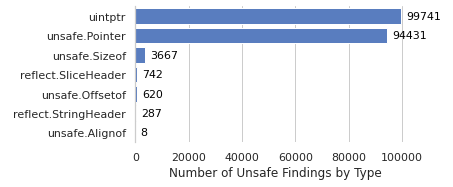
\includegraphics[width=0.5\textwidth]{gfx/figures/distribution-unsafe-types.png}
    \caption{Distribution of different types of unsafe token types. Answers \ref{rq:distTypes}}
    \label{fig:unsafe-tokens-distribution}
\end{figure}

\begin{figure*}[ht]
    \centering
    {\scriptsize 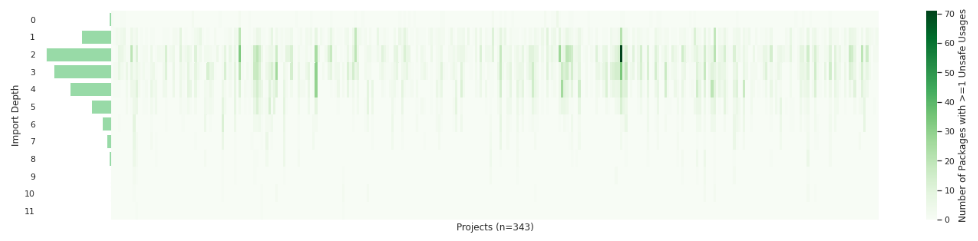
\includegraphics[width=\textwidth,height=6cm]{gfx/figures/unsafe-import-depth.tikz}}
    \caption{Import Depth of Unsafe Packages. Answers \ref{rq:depsDepth}: unsafe packages are around \checkNum{3.5 $\pm 2$} hops away, thus manageable to find manually. \jl{Add mean and deviation}}
    \label{fig:unsafe-import-depth}
\end{figure*}

\begin{figure*}[ht]
    \centering
    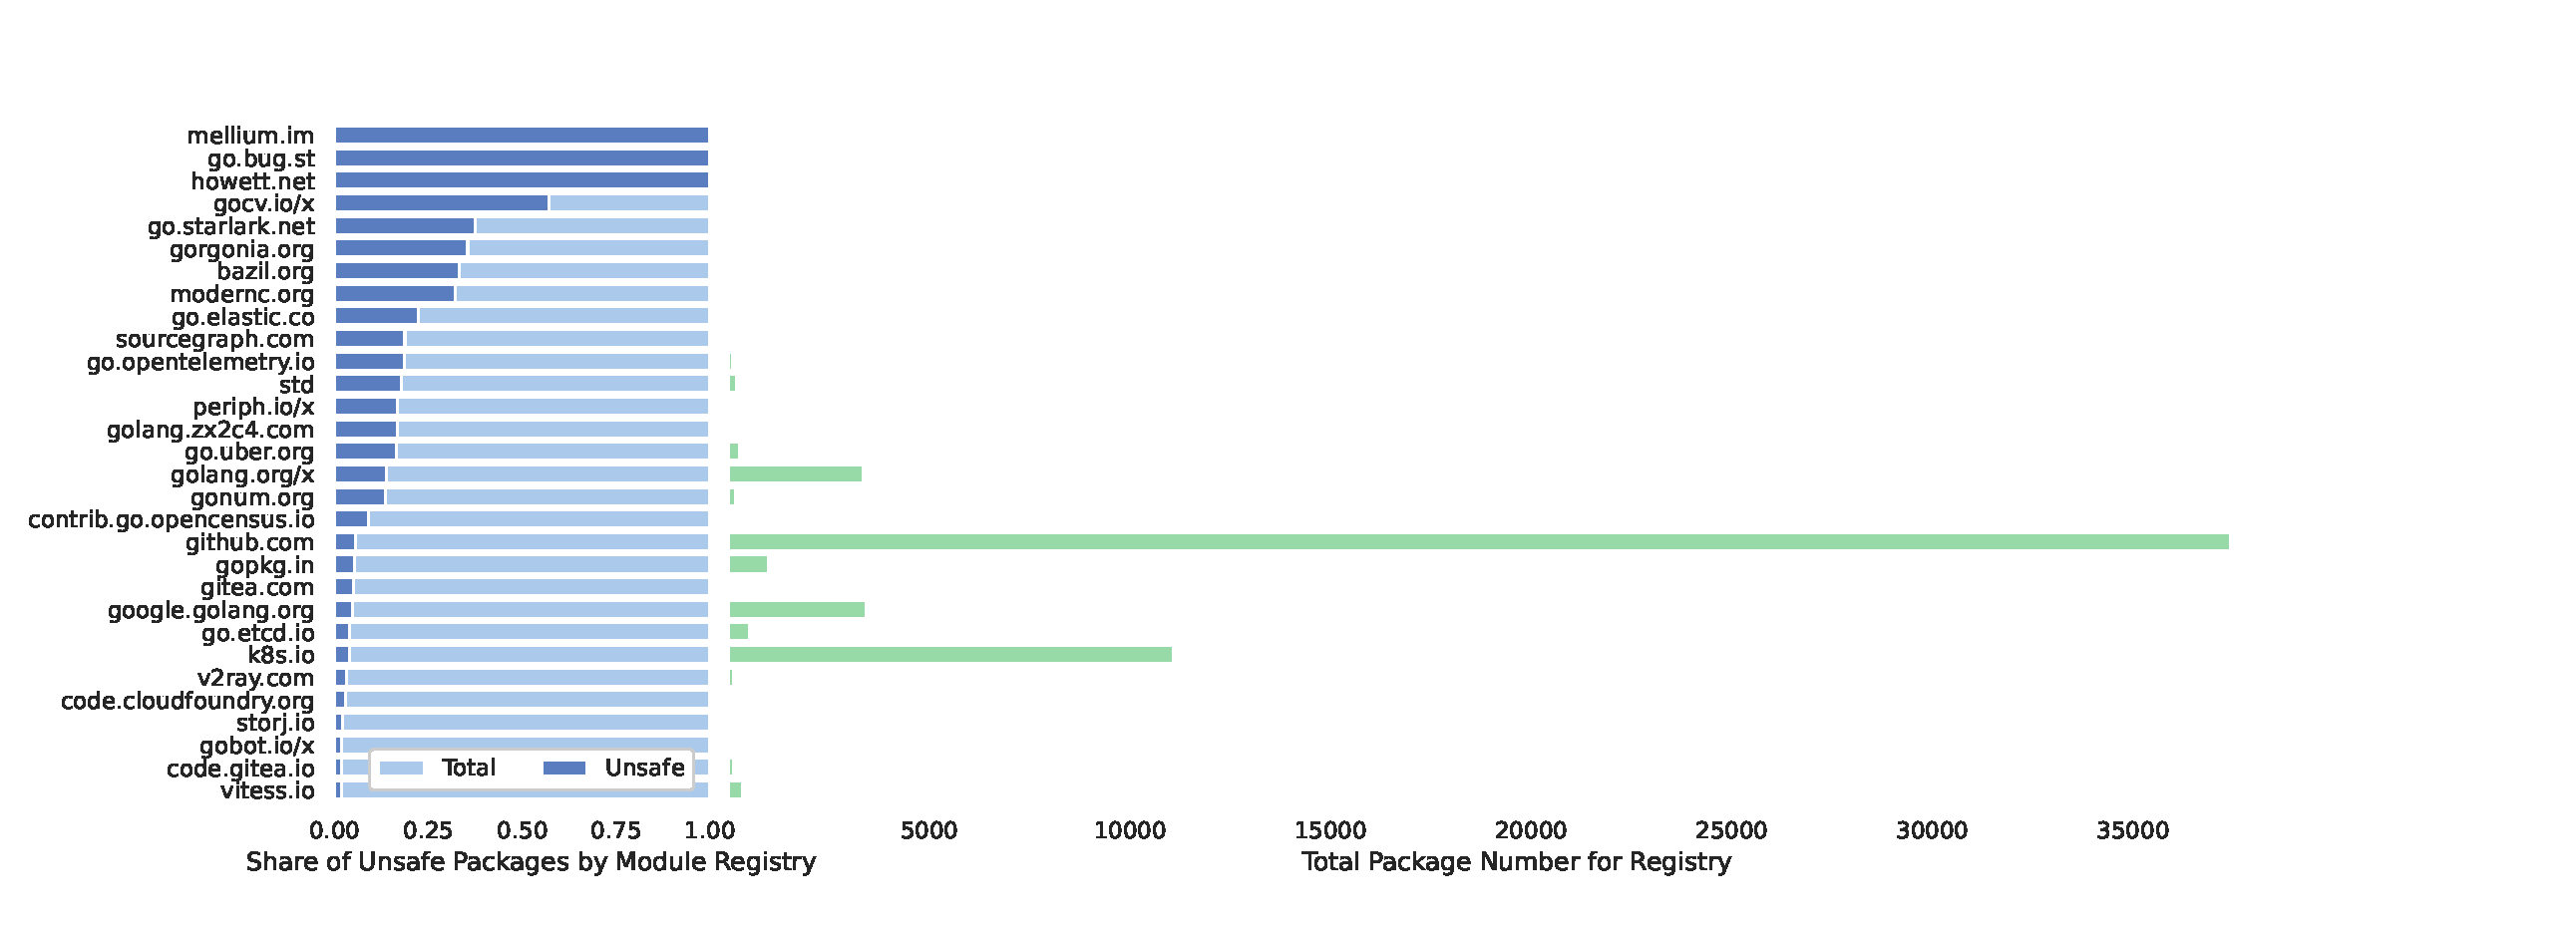
\includegraphics[width=\textwidth]{gfx/figures/unsafe-packages-by-registry-n30.eps}
    \caption{Share of Unsafe Packages by Registry along with Total Package Count for Registries, Showing the Top \checkNum{30} Registries by Unsafe Share. Answers \ref{rq:prevalDeps} in its current form}
    \label{fig:unsafe-by-registry}
\end{figure*}

\begin{table}[h]
    \centering
    \caption{Selected projects for creation of the labeled data set}
    \label{tbl:dataset-projects}
    \begin{tabular}{llrrll}
    \hline
        {}  &                                               Name &  Stars &  Forks &   Revision \\ \hline
        1   &                              kubernetes/kubernetes &  66512 &  23806 &  fb9e1946b0 \\
        2   &                       mattermost/mattermost-server &  18277 &   4157 &  e83cc7357c \\
        3   &                                    rancher/rancher &  14344 &   1758 &  56a464049e \\
        4   &                                   weaveworks/scope &   4354 &    554 &  bf90d56f0c \\
        5   &                                          rook/rook &   7208 &   1472 &  ff90fa7098 \\
        6   &                                      elastic/beats &   8852 &   3207 &  df6f2169c5 \\
        7   &                                hashicorp/terraform &  22151 &   5729 &  01f91316da \\
        8   &                                      cilium/cilium &   5501 &    626 &  9b0ae85b5f \\
        9   &                                       grafana/loki &   9537 &    922 &  10a1f28a85 \\
        10  &                                  gorgonia/gorgonia &   3373 &    301 &  5fb5944d4a \\
        \hline
    \end{tabular}
\end{table}

\begin{table*}[t]
    \centering
    \caption[Labeled unsafe.Pointer usages in application code samples Answers \ref{rq:purpose}]%
    {Labeled unsafe.Pointer usages in application code samples \newline \tiny ~ \newline \small
        \underline{eff}: efficiency, \underline{gen}: generics, \underline{ser}: (de)serialization,
        \underline{inev}: inevitable use, \underline{SR}: safer reflections, \underline{LC}: layout control,
        \underline{EA}: hide from escape analysis, \underline{UU}: unused,
        \underline{doc}: documentation \newline \tiny ~}
    \label{tbl:dataset-classes-app}
    \begin{tabular}{r|ccccccccc|r}
                                          &  eff &  gen & ser & inev &  SR &  LC &  EA &  UU & doc &  {}   \\ \hline
                 conversion-struct-struct &  396 &   58 &   7 &    2 &   2 &   1 &    &     &     &   466 \\
        \rowcolor{verylightgray}
                  conversion-struct-basic &   80 &   35 &   5 &      &     &   1 &    &     &     &   121 \\
                        conversion-header &   26 &    8 &   3 &      &     &     &    &     &     &    37 \\
        \rowcolor{verylightgray}
                  conversion-struct-bytes &   21 &    1 &  70 &    1 &     &   3 &    &     &     &    96 \\
                     direct-memory-access &    9 &   19 &     &    9 &   1 &   1 &    &     &     &    39 \\
        \rowcolor{verylightgray}
                       pointer-arithmetic &    7 &    2 &   1 &      &     &   7 &  1 &     &     &    18 \\
                           data-structure &    7 &    5 &     &    2 &  22 &   1 &    &   1 &     &    38 \\
        \rowcolor{verylightgray}
                                 delegate &    4 &   63 &   1 &   19 &   1 &     &    &     &     &    88 \\
                          type-reflection &      &   32 &     &      &   2 &     &    &     &     &    34 \\
        \rowcolor{verylightgray}
                                  syscall &      &      &     &   21 &     &     &    &     &     &    21 \\
                                   unused &      &      &     &      &     &     &    &  15 &     &    15 \\
        \rowcolor{verylightgray}
                                  comment &      &      &     &      &     &     &    &  23 &   4 &    27 \\ \hline
                                       {} &  550 &  223 &  87 &   54 &  28 &  14 &  1 &  39 &   4 &  1000 \\
    \end{tabular}
\end{table*}

\begin{table*}[t]
    \centering
    \caption[Labeled unsafe.Pointer usages in standard library samples. Answers \ref{rq:purpose}]%
        {Labeled unsafe.Pointer usages in standard library samples \newline \tiny ~ \newline \small
            \underline{no GC}: avoid garbage collector, \underline{typ}: types implementation,
            \underline{mem}: memory management, \underline{inev}: inevitable use, \underline{eff}: efficiency,
            \underline{ser}: (de)serialization, \underline{LC}: layout control, \underline{cgo}: CGo mechanics,
            \underline{EA}: hide from escape analysis, \underline{UU}: unused, \underline{UU}: unnecessary use \newline \tiny ~}
    \label{tbl:survey-small-results-std}
    \begin{tabular}{r|ccccccccccc|r}
                                          & no GC & typ & mem & inev & eff & ser & LC & cgo & EA & UN & UU &   {} \\ \hline
                                  syscall &   151 &     &     &    3 &     &     &    &     &    &  1 &    &  155 \\
        \rowcolor{verylightgray}
                     direct-memory-access &       &  10 &  13 &      &  17 &   2 &  2 &     &    &    &    &   44 \\
                       pointer-arithmetic &       &   9 &   7 &    2 &   5 &     &  4 &   1 &  1 &    &    &   29 \\
        \rowcolor{verylightgray}
                 conversion-struct-struct &       &  20 &   4 &    4 &   1 &   9 &    &   1 &  1 &    &    &   40 \\
                  conversion-struct-basic &       &     &   3 &    1 &     &   2 &  2 &   1 &    &    &    &    9 \\
        \rowcolor{verylightgray}
                        conversion-header &       &   2 &   1 &      &     &     &    &     &    &    &    &    3 \\
                  conversion-struct-bytes &       &     &     &      &   4 &   8 &    &     &    &    &    &   12 \\
        \rowcolor{verylightgray}
                           data-structure &       &   7 &  11 &    1 &     &     &    &   3 &    &    &    &   22 \\
                                 delegate &       &   4 &  16 &   47 &     &     &    &     &  6 &    &    &   73 \\
        \rowcolor{verylightgray}
                          type-reflection &       &   3 &     &      &     &   1 &    &     &    &    &    &    4 \\
                                   unused &       &     &     &      &     &     &    &     &    &    &  8 &    8 \\
        \rowcolor{verylightgray}
                                  comment &       &     &     &      &     &     &    &     &    &    &  1 &    1 \\ \hline
                                       {} &   151 &  55 &  55 &   58 &  27 &  22 &  8 &   6 &  8 &  1 &  9 &  400 \\
    \end{tabular}
\end{table*}

\textbf{Answers to research questions:}

\checkNum{3355} of \checkNum{61839} (\checkNum{5.43\%}) transitively imported packages use unsafe. This answers \ref{rq:prevalDeps}

Number of projects: \checkNum{343}

Projects with $\geq 1$ unsafe project package: \checkNum{131} (\checkNum{38.19\%})

Projects with $\geq 1$ unsafe dependency: \checkNum{299} (\checkNum{87.17\%})

Projects with $\geq 1$ unsafe anywhere: \checkNum{312} (\checkNum{90.96\%})

These answer \ref{rq:prevalApp} and \ref{rq:prevalDeps}.

\section{Exploit Proof of Concepts}
\label{sec:exploits}

\section{Tools to Help Developers}
\label{sec:tools}

\aw{Why not discuss this in related work?}
\section{Discussion}
\label{sec:discussion}

\begin{itemize}
    \item exploit-ability is not only of academic nature
\end{itemize}

\section{Conclusion}
\label{sec:concl}


% conference papers do not normally have an appendix

% use section* for acknowledgment
\ifCLASSOPTIONcompsoc
  % The Computer Society usually uses the plural form
  \section*{Acknowledgments}
\else
  % regular IEEE prefers the singular form
  \section*{Acknowledgment}
\fi

The authors would like to thank...



% trigger a \newpage just before the given reference
% number - used to balance the columns on the last page
% adjust value as needed - may need to be readjusted if
% the document is modified later
%\IEEEtriggeratref{8}
% The "triggered" command can be changed if desired:
%\IEEEtriggercmd{\enlargethispage{-5in}}

% references section

% can use a bibliography generated by BibTeX as a .bbl file
% BibTeX documentation can be easily obtained at:
% http://mirror.ctan.org/biblio/bibtex/contrib/doc/
% The IEEEtran BibTeX style support page is at:
% http://www.michaelshell.org/tex/ieeetran/bibtex/
\bibliographystyle{IEEEtran}
% argument is your BibTeX string definitions and bibliography database(s)
\bibliography{IEEEabrv,references}

% that's all folks
\end{document}
